\documentclass[12pt, twoside]{article}
\usepackage[letterpaper, margin=1in, headsep=0.5in]{geometry}
\usepackage[english]{babel}
\usepackage[utf8]{inputenc}
\usepackage{amsmath}
\usepackage{amsfonts}
\usepackage{amssymb}
\usepackage{tikz}
\usetikzlibrary{quotes, angles}
\usepackage{graphicx}
\usepackage{enumitem}
\usepackage{multicol}

\newif\ifmeta
\metatrue %print standards and topics tags

\title{Regents Geometry}
\author{Chris Huson}
\date{December 2021}

\usepackage{fancyhdr}
\pagestyle{fancy}
\fancyhf{}
\renewcommand{\headrulewidth}{0pt} % disable the underline of the header
\raggedbottom

\fancyhead[LE]{\thepage}
\fancyhead[RO]{\thepage \\ Name: \hspace{4cm} \,\\}
\fancyhead[LO]{BECA / Dr. Huson / Geometry 5 Congruence Transformations}

\begin{document}

\subsubsection*{5.1 Classwork: Translation \hfill CCSS.HSG.CO.A.5}
\begin{enumerate}
  \item Slide the point $A(2)$ two units to the right. Mark and label it $A'$. What slide would shift $A$ onto the point $B(-3)$?
  \begin{flushright}
      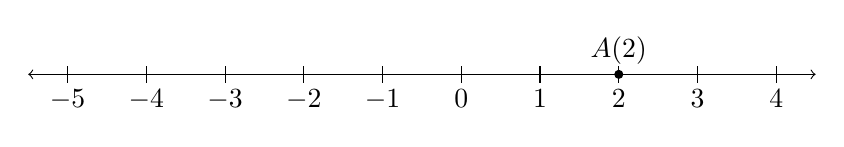
\begin{tikzpicture}
        \draw [<->] (-5.5,0)--(4.5,0);
        \foreach \x in {-5,...,4}
          \draw[shift={(\x,0)},color=black] (0pt,-3pt) -- (0pt,3pt) node[below=5pt]  {$\x$};
          \draw [fill] (2,0) circle [radius=0.05] node[above] {$A(2)$};
      \end{tikzpicture}
    \end{flushright}
    
  \item On the axes below, graph the point $N(-3,2)$ and its image, $N'$, after a translation of right 3, down 4. Mark $N'$ and write it down as a coordinate pair.
  \begin{center}
    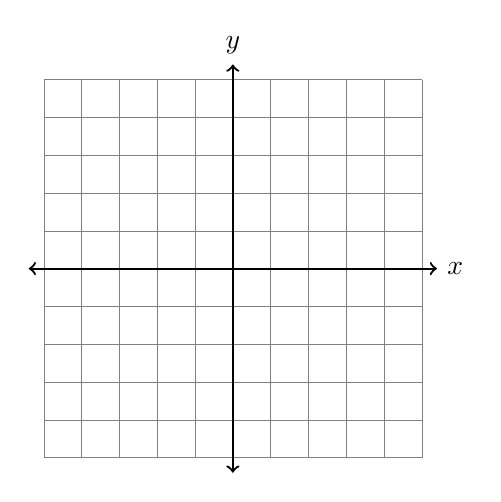
\begin{tikzpicture}[scale=.48]
    \draw [help lines] (-5,-5) grid (5,5);
    \draw [thick, <->] (-5.4,0) -- (5.4,0) node [right] {$x$};
    \draw [thick, <->] (0,-5.4)--(0,5.4) node [above] {$y$};   
  \end{tikzpicture}
\end{center}

\item Apply the translation $(x,y) \rightarrow (x-3,y+5)$ to the point $P(-2,-5)$. \vspace{2cm}

\item Identify the transformation that maps $\triangle ABC$ onto its image $\triangle A'B'C'$.
\begin{flushright}
    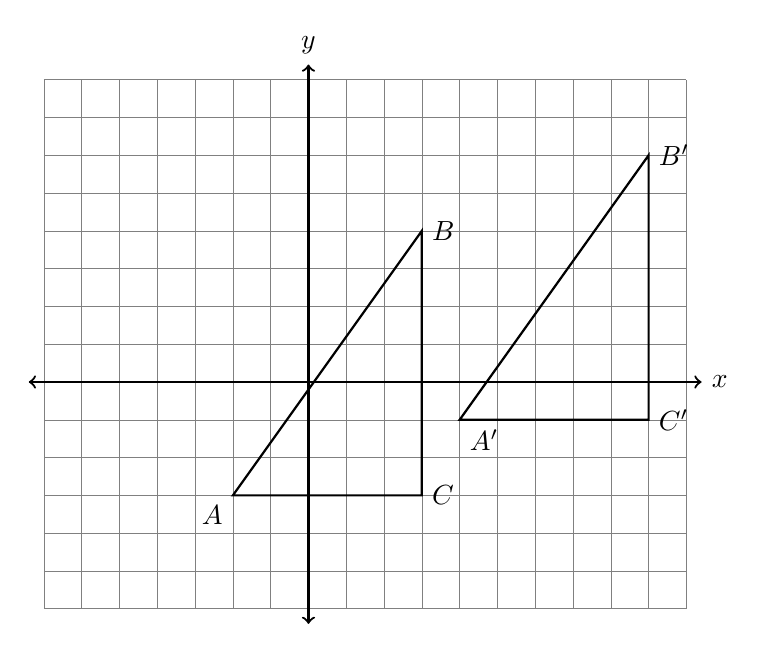
\begin{tikzpicture}[scale=.48]
    \draw [help lines] (-7,-6) grid (10,8);
    \draw [thick, <->] (-7.4,0) -- (10.4,0) node [right] {$x$};
    \draw [thick, <->] (0,-6.4)--(0,8.4) node [above] {$y$};  
    \draw [thick]
      (-2,-3) node[below left] {$A$}--
      (3,4) node[right] {$B$}--
      (3,-3) node[right] {$C$}--cycle;  
    \draw [thick]
      (4,-1) node[below right] {$A'$}--
      (9,6) node[right] {$B'$}--
      (9,-1) node[right] {$C'$}--cycle;   \end{tikzpicture}
\end{flushright}

\newpage
\item Slide $\triangle ABC$ to the left four and up five. Label the image $\triangle A'B'C'$.
  \begin{center}
      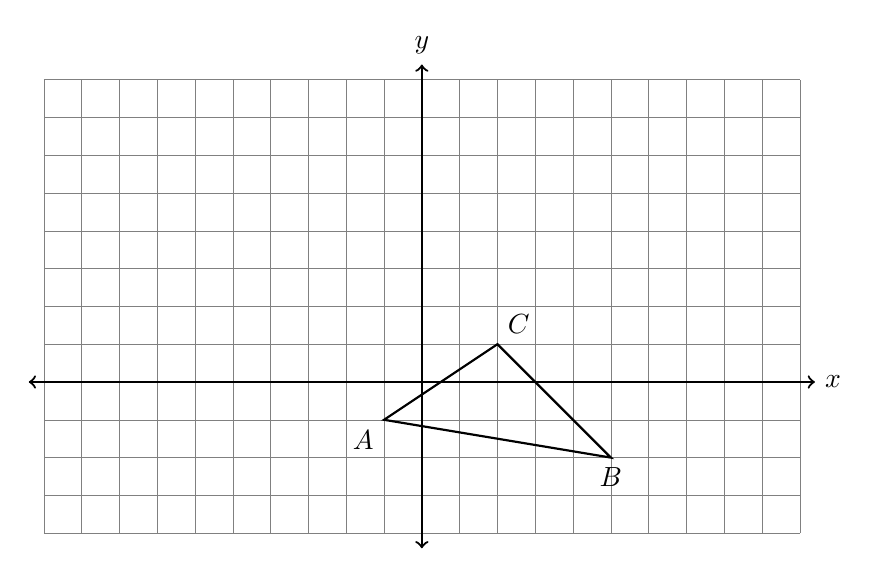
\begin{tikzpicture}[scale=.48]
      \draw [help lines] (-10,-4) grid (10,8);
      \draw [thick, <->] (-10.4,0) -- (10.4,0) node [right] {$x$};
      \draw [thick, <->] (0,-4.4)--(0,8.4) node [above] {$y$};  
      \draw [thick]
        (-1,-1) node[below left] {$A$}--
        (5,-2) node[below] {$B$}--
        (2,1) node[above right] {$C$}--cycle;  
    \end{tikzpicture}
  \end{center}
 
\item State the translation that would map $Q(4,3)$ onto $Q'(-1,-3)$. \vspace{2cm}

\item Triangle $A'B'C'$ is the image of triangle $ABC$ after a translation of 2 units to the right and 3 units up. Is triangle $ABC$ congruent to $A'B'C'$? Explain why. \vspace{3cm}
 
\item State the translation that would map $C(-4,0)$ onto $C'(3,-3)$. (the use of the grid below is optional)
\begin{center}
  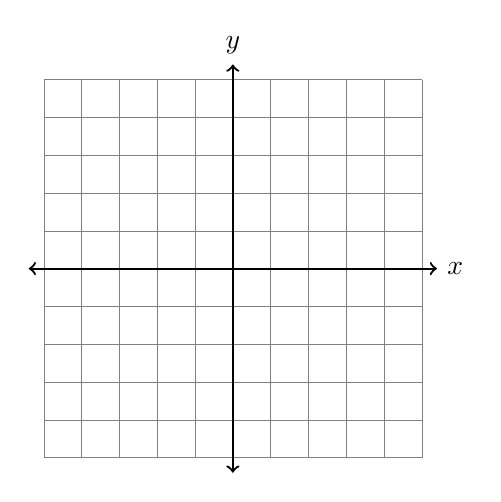
\begin{tikzpicture}[scale=.48]
  \draw [help lines] (-5,-5) grid (5,5);
  \draw [thick, <->] (-5.4,0) -- (5.4,0) node [right] {$x$};
  \draw [thick, <->] (0,-5.4)--(0,5.4) node [above] {$y$};   
\end{tikzpicture}
\end{center}

\item On the axes below, plot the point $A(-4,-1)$ and its image, $A'$, after the translation $(x,y) \rightarrow (x+6,y-3)$. Label the image as a coordinate pair.
    \begin{center}
      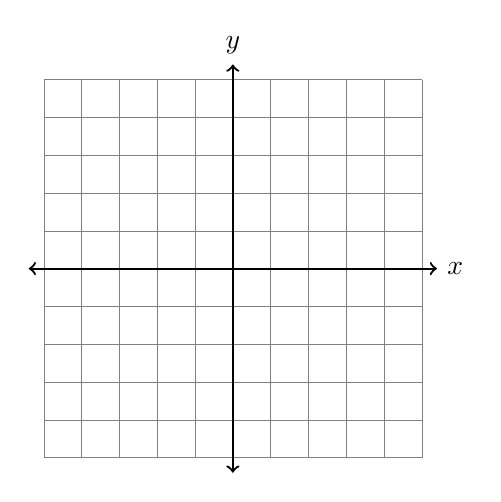
\begin{tikzpicture}[scale=.48]
      \draw [help lines] (-5,-5) grid (5,5);
      \draw [thick, <->] (-5.4,0) -- (5.4,0) node [right] {$x$};
      \draw [thick, <->] (0,-5.4)--(0,5.4) node [above] {$y$};   
    \end{tikzpicture}
  \end{center}

  \item The image of triangle $ABC$ after a translation is $\triangle A'B'C'$. Is the area of the triangle greater, smaller, or the same after the translation? Justify your answer. \vspace{3cm}


\end{enumerate}
\end{document}